\documentclass{beamer}
\usepackage[utf8]{inputenc}
\usepackage[T1]{fontenc}
\usepackage[portuges,brazilian]{babel}
\usepackage{graphicx}
\usepackage[sfdefault]{quattrocento}
\usepackage{multicol}
\usepackage{hyperref}
\usepackage[alf]{abntex2cite}
\usepackage{color}
\useoutertheme{infolines}
\useinnertheme{rectangles}
\usefonttheme{professionalfonts}

\title{Módulo de pré visualização para a ferramenta CGT}
\subtitle{Ceará Game Tools}
\author[Joel]{Joel Rocha}
\institute[IFCE]{Orientador: Prof. Dr. Carlos Hairon
   \par Engenharia de Computação
   \par Instituto Federal de Ciência, Arte e Tecnologia}
\date{Dezembro, 2015}
\logo{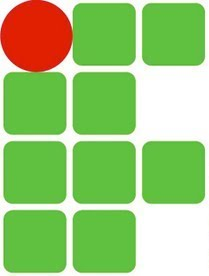
\includegraphics[width=0.8cm]{images/logo.jpg}}

\begin{document}
   \begin{frame}
      \titlepage
   \end{frame}

   \begin{frame}{\contentsname}
      \begin{multicols}{2}
         {\footnotesize \tableofcontents}
      \end{multicols}
   \end{frame}

   \section{Introdução}
   \subsection{Indústria de jogos digitais}
   \begin{frame}
      \frametitle{Introdução}
      \framesubtitle{Qual a importância dos jogos?}
      \begin{itemize}
         \item Geração de emprego e renda {\scriptsize (produtor, desenvolvedor, testador, \emph{designer}, roteirista, dublador)}.
         \item Inovação tecnológica.
         \item Diversidade no público alvo.
         \item Várias plataformas (PC, Console, Mobile).
         \item Movimenta em torno de US\$ 82 bilhões. \cite{ind-bra-relatorio}
      \end{itemize}
   \end{frame}
   \begin{frame}
      \begin{center}
         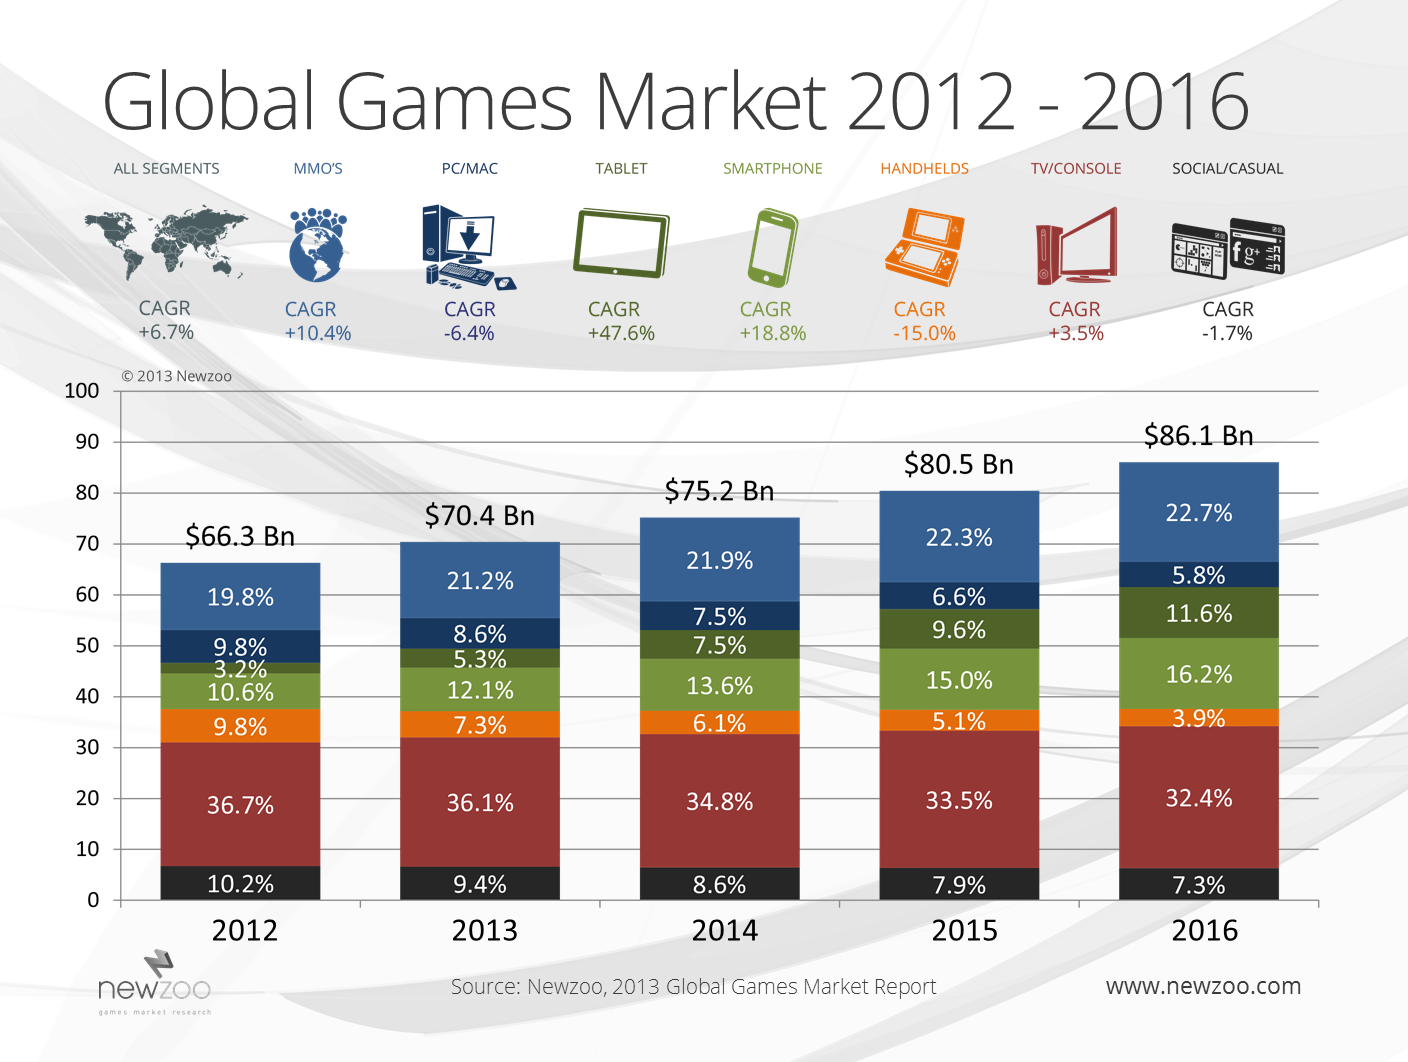
\includegraphics[width=\textwidth]{images/Newzoo_Global_Games_Market_2012-2016_V1.png}
      \end{center}
   \end{frame}
   \subsection{Projeto CGT}
   \begin{frame}
      \frametitle{Introdução}
      \framesubtitle{O que é o Projeto CGT?}
      Projeto Ceará \emph{Games Tools} tem o objetivo de oferecer uma ferramenta para a construção de jogos onde qualquer um poderá criar seu próprio jogo. \cite{website:projeto-cgt}
   \end{frame}
   \subsection{Vínculo CNPQ}
   \begin{frame}
      \frametitle{Introdução}
      \framesubtitle{Projeto CGT e o CNPQ}
      \begin{itemize}
         \item Pesquisa, Desenvolvimento e Comercialização de Games Temáticos da Cultura Cearense.
         \item Edital 80 de 2013, processo 409227/2013-7.
         \item \emph{Software livre}.
         \item Multiplataforma.
      \end{itemize}
   \end{frame}
   \subsection{Projeto de extensão}
   \begin{frame}
      \begin{columns}[T]
         \begin{column}{0.48\textwidth}
            \frametitle{Introdução}
            \framesubtitle{Projeto de extensão}
            \begin{itemize}
               \item Curso de desenvolvimento de jogos digitais;
               \item Para 14 jovens do ensino fundamental e médio;
               \item Difundir a cultura do desenvolvimento de jogos;
               \item Ferramentas de desenvolvimento:
                  \begin{itemize}
                     \item Construct 2 e
                     \item Ferramenta CGT (versão 2.0).
                  \end{itemize}
            \end{itemize}
         \end{column}
         \begin{column}{0.48\textwidth}
            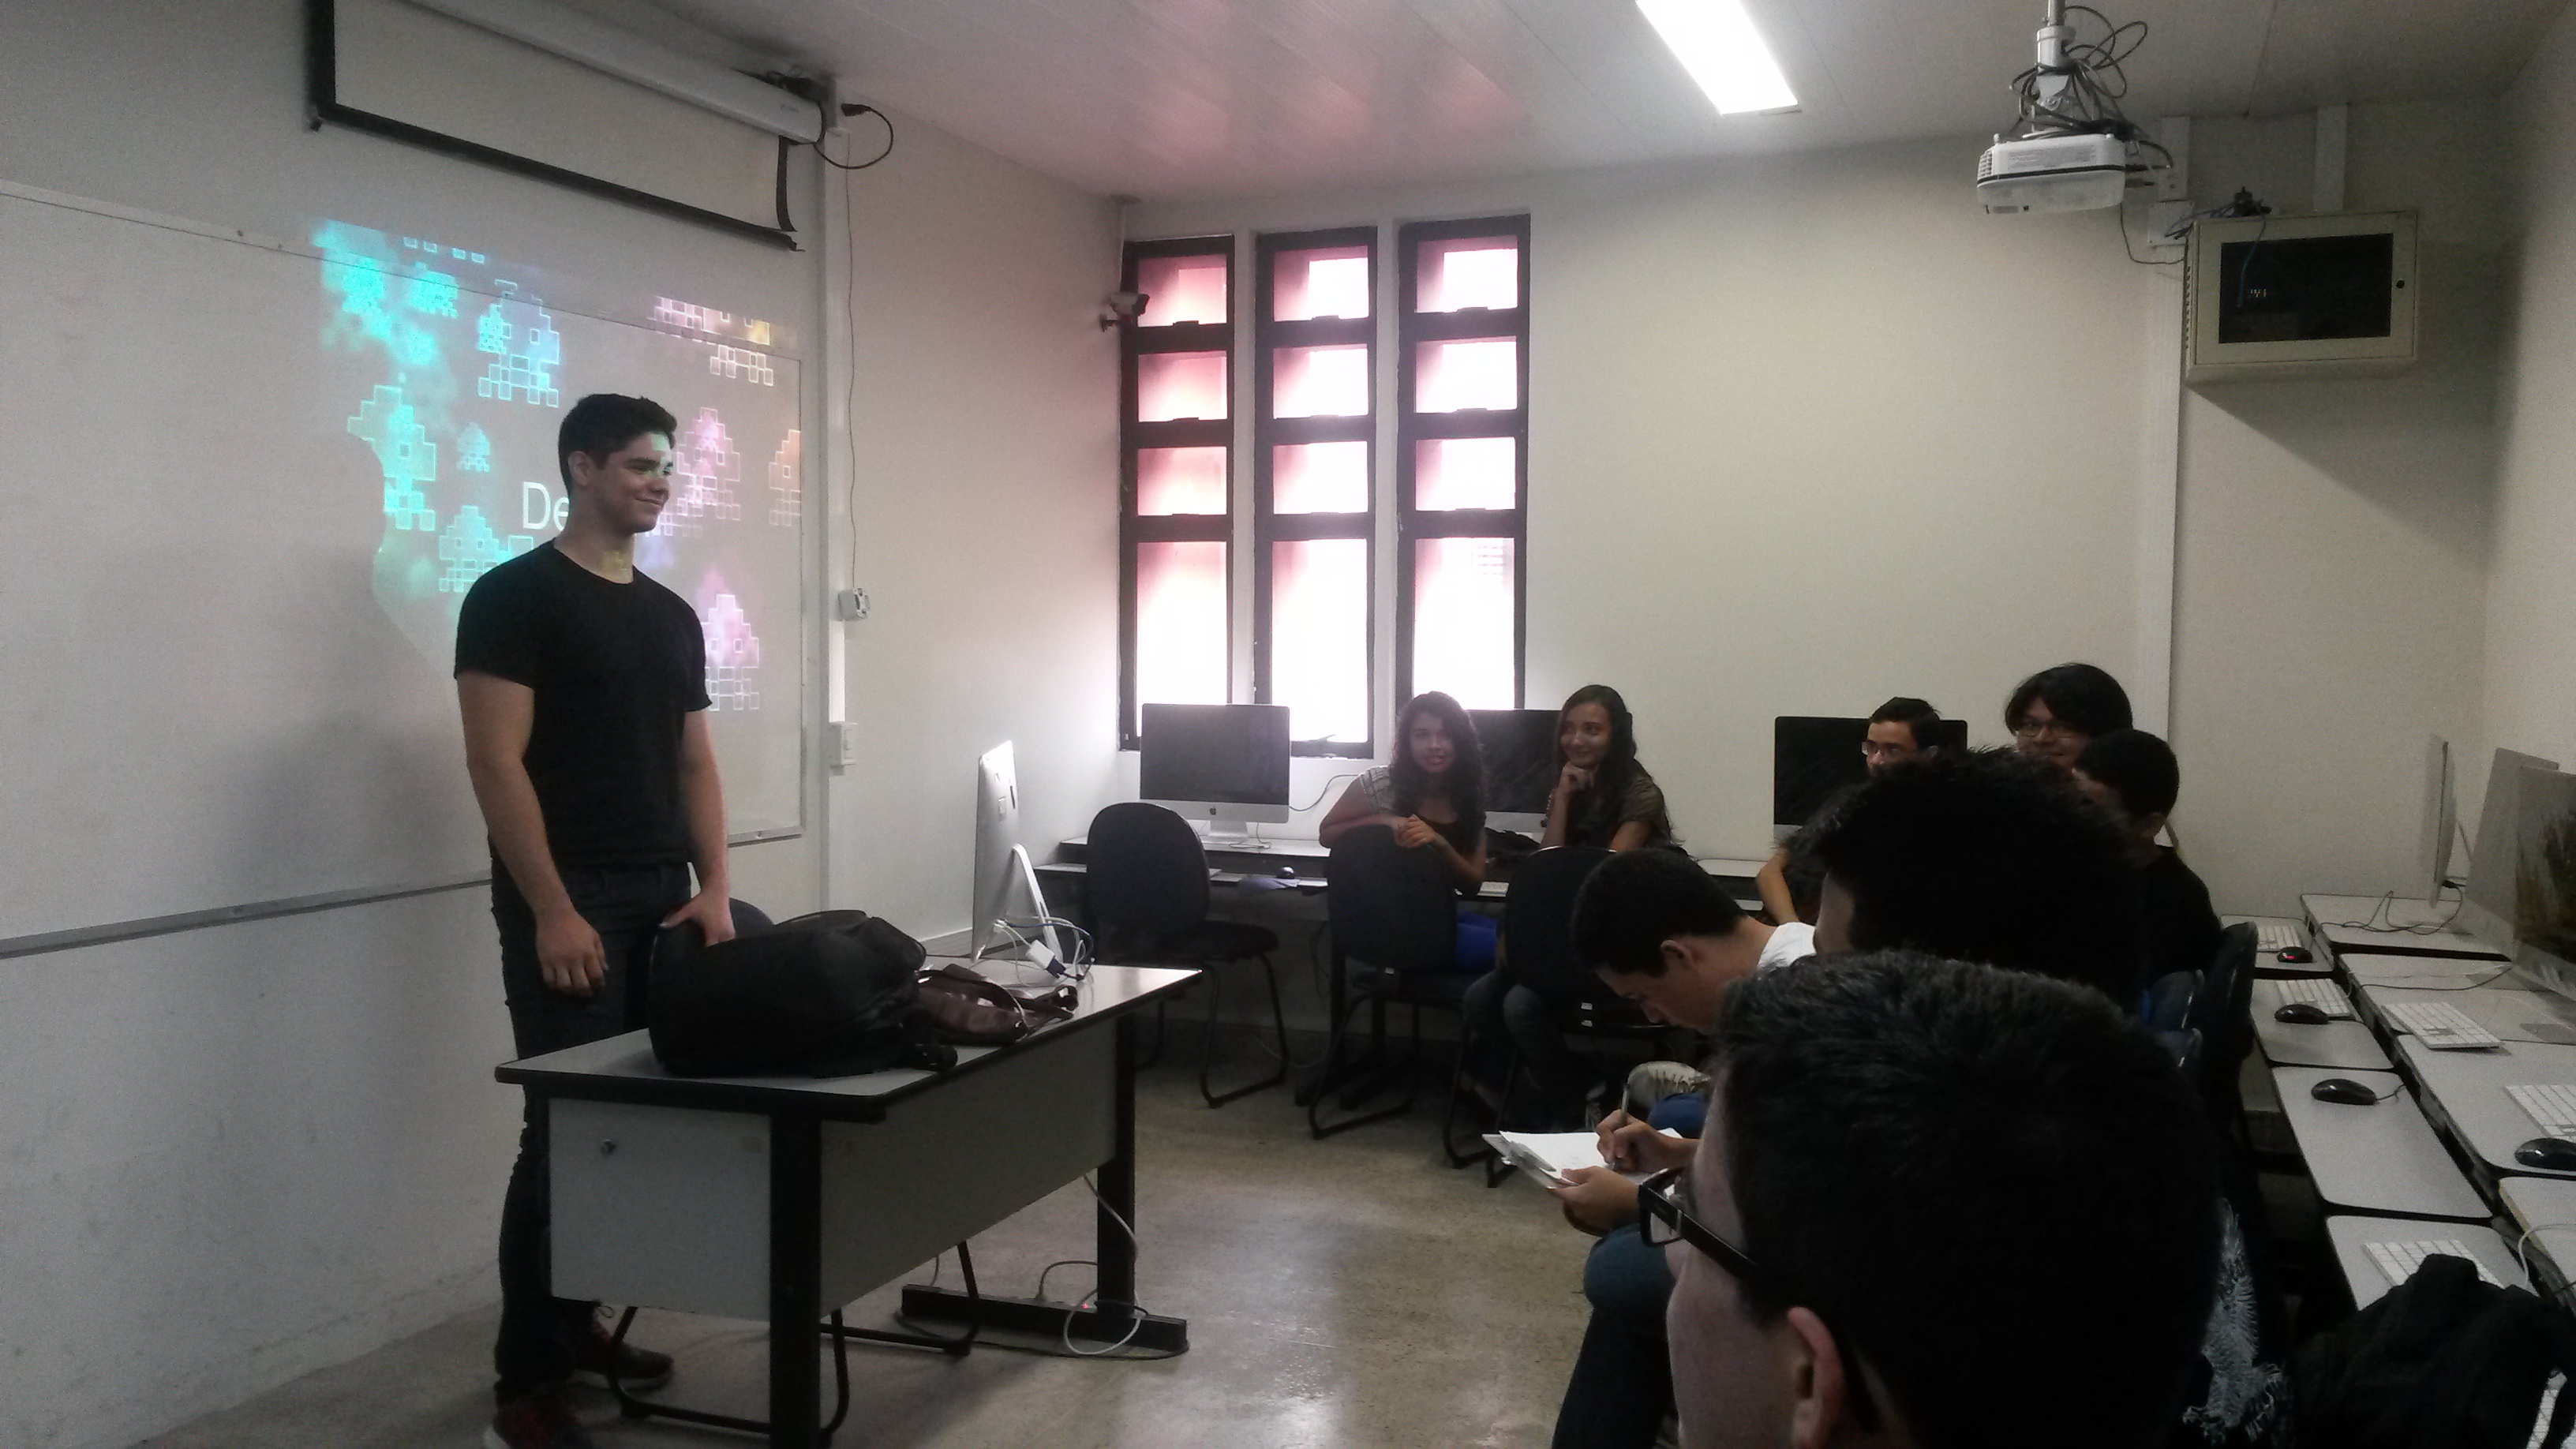
\includegraphics[width=\textwidth]{images/ext/20150921_101616.jpg}
         \end{column}
      \end{columns}
   \end{frame}

   \begin{frame}
      \frametitle{Introdução}
      \framesubtitle{Retorno dos usuários}
      \begin{columns}[T]
         \begin{column}{0.48\textwidth}
            \begin{itemize}
               \item Fácil aprendizagem;
               \item Correção de erros;
               \item 93\% dos usuários preferem a ferramenta CGT;
               \item Motivos:
                  \begin{itemize}
                     \item Idioma;
                     \item Simplicidade e
                     \item Recursos disponíveis.
                  \end{itemize}
            \end{itemize}
         \end{column}
         \begin{column}{0.48\textwidth}
            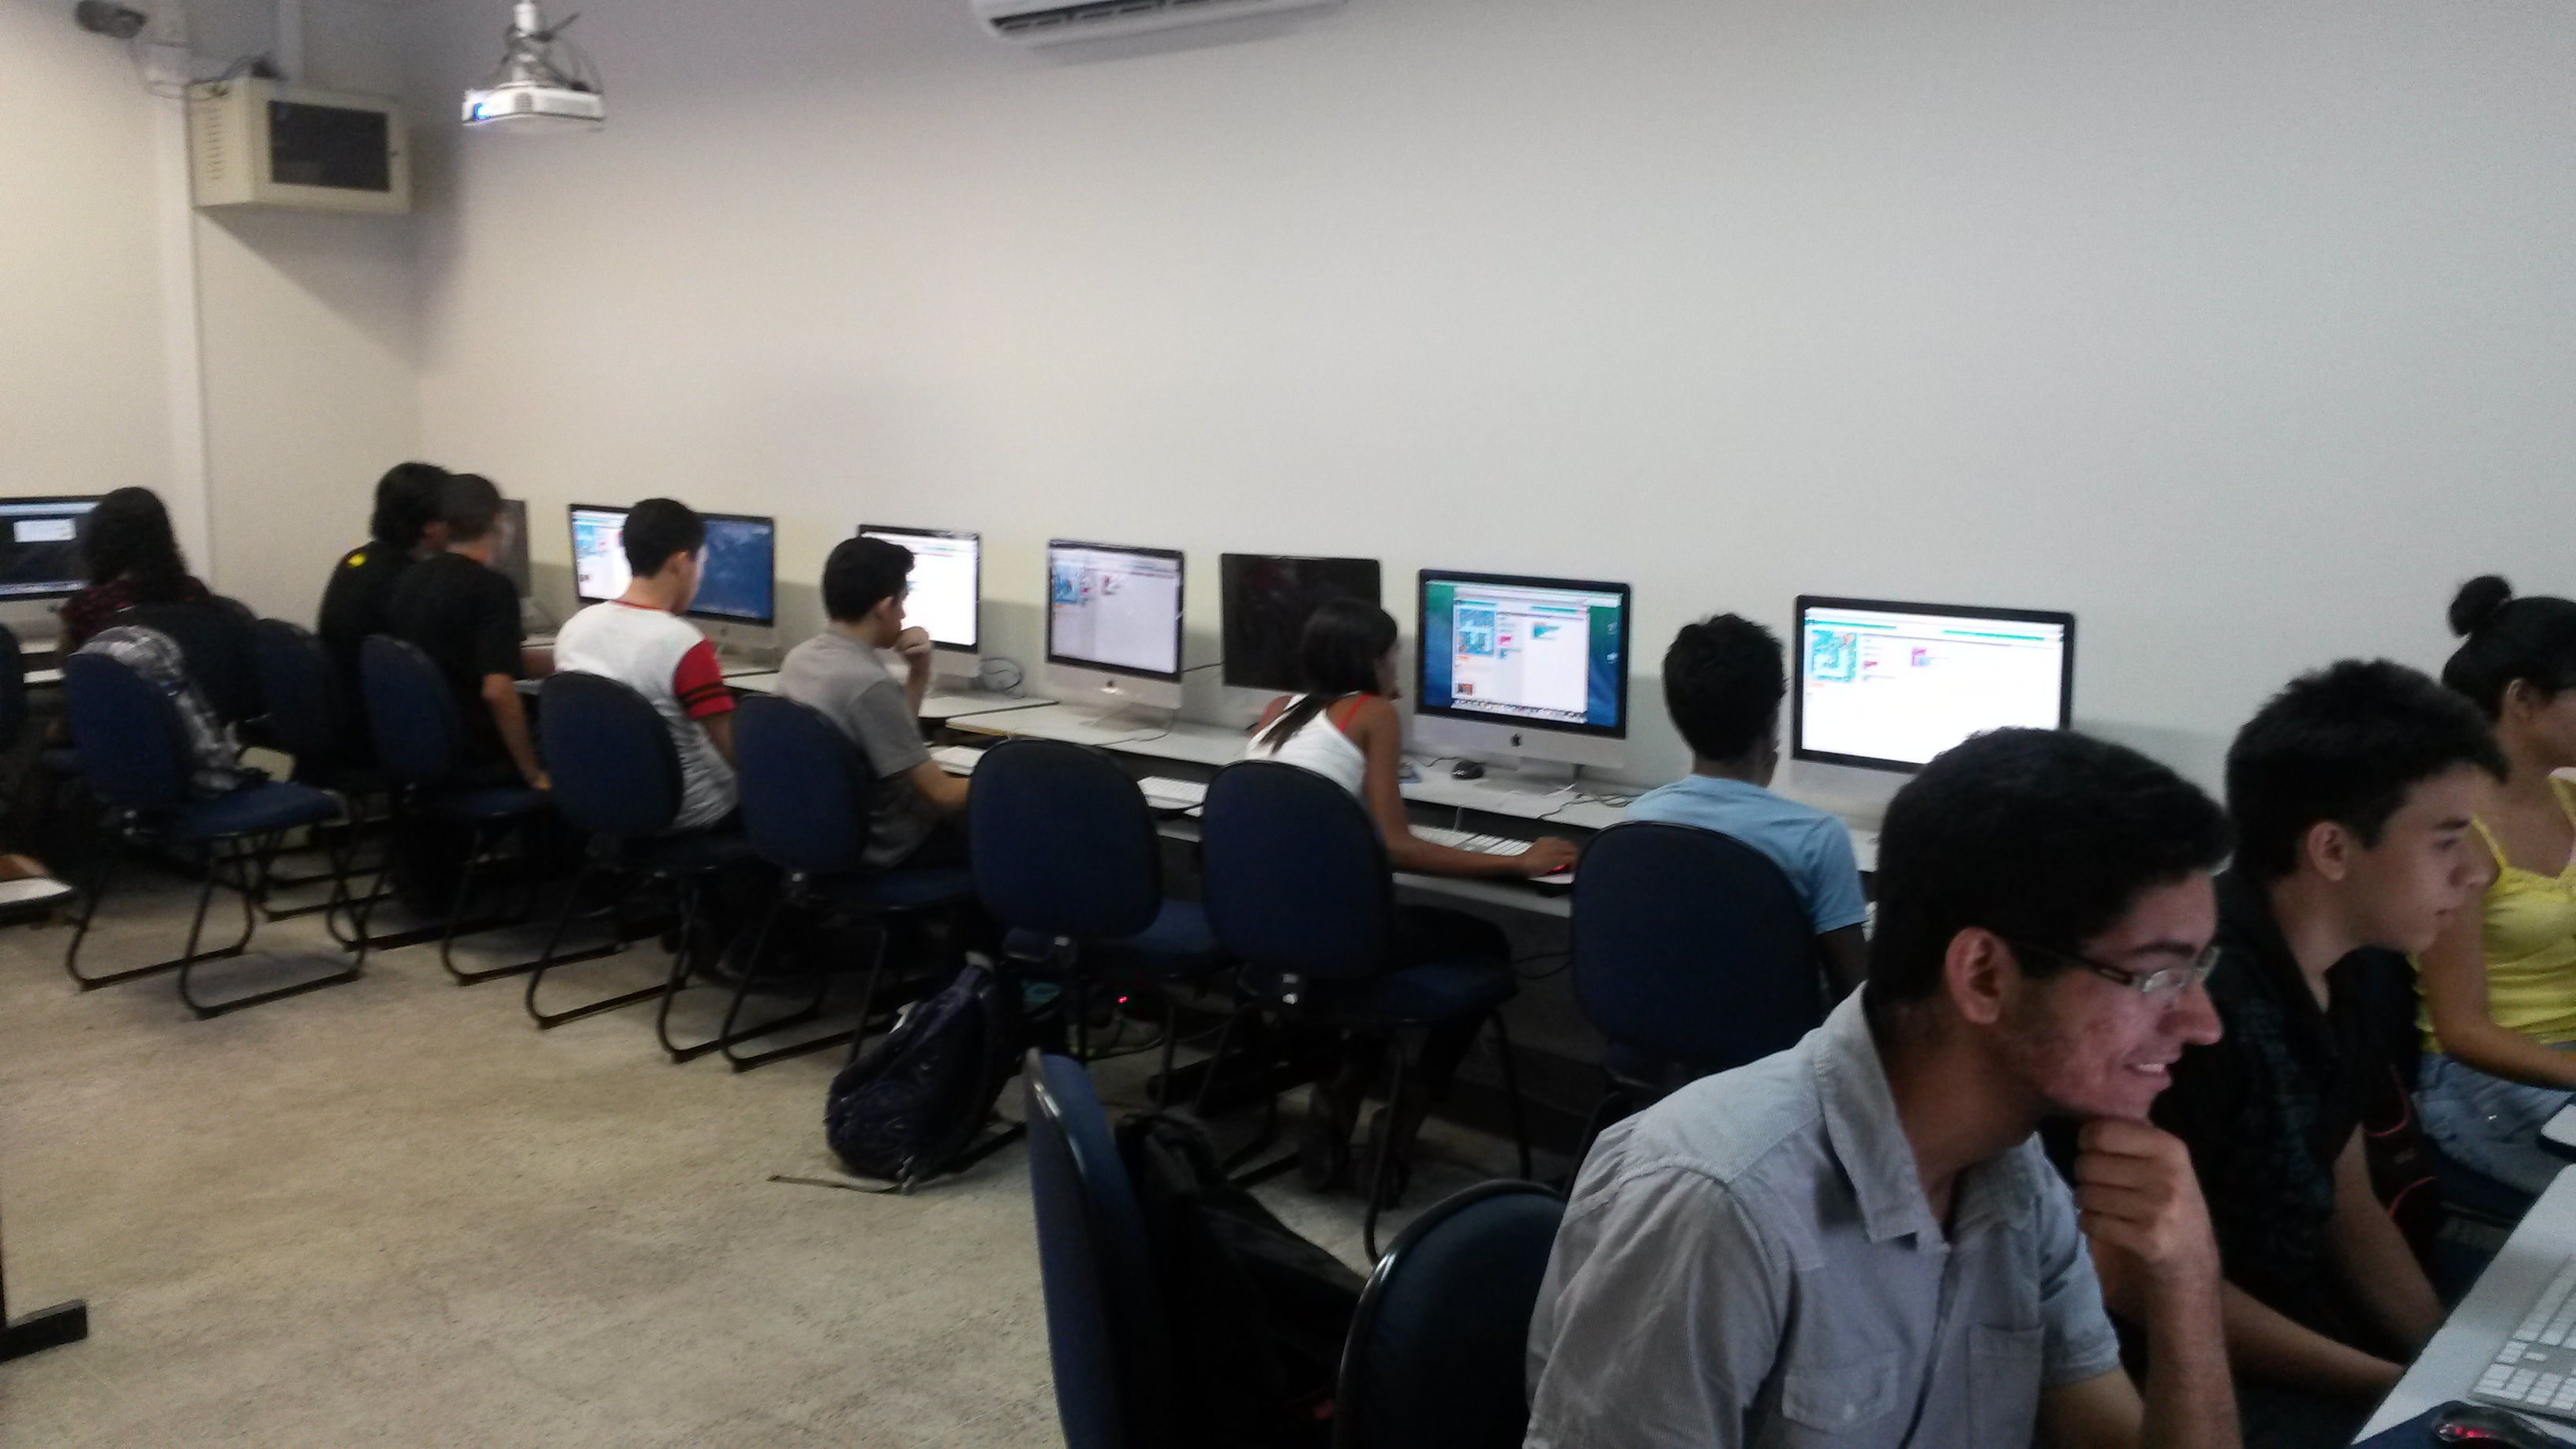
\includegraphics[width=\textwidth]{images/ext/20150902_110944.jpg}
         \end{column}
      \end{columns}
   \end{frame}

   \subsection{Introdução ao problema}
   \begin{frame}
      \frametitle{Introdução}
      \framesubtitle{Problemas da ferramenta 1.0}
      \begin{itemize}
         \item Controles confusos;
         \item Ausência de \emph{feedback};
         \item \textbf{Pré visualização.}
      \end{itemize}
   \end{frame}
   \begin{frame}
      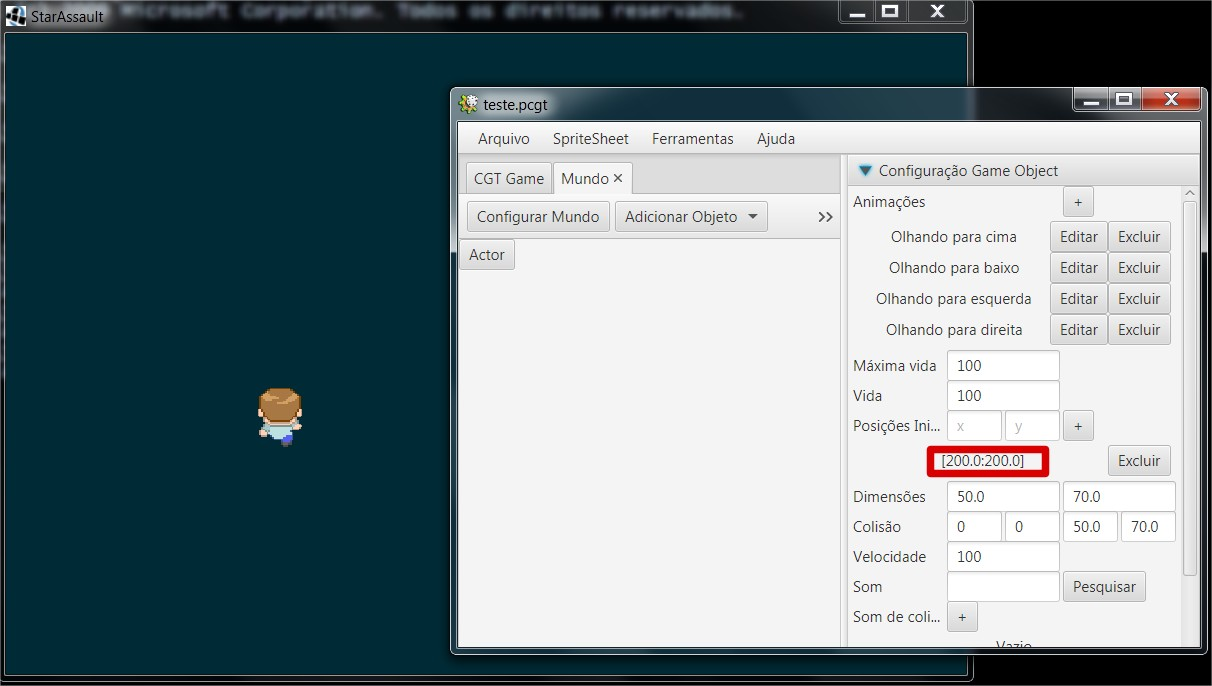
\includegraphics[width=\textwidth]{images/problema-1.jpg}
   \end{frame}

   \begin{frame}
      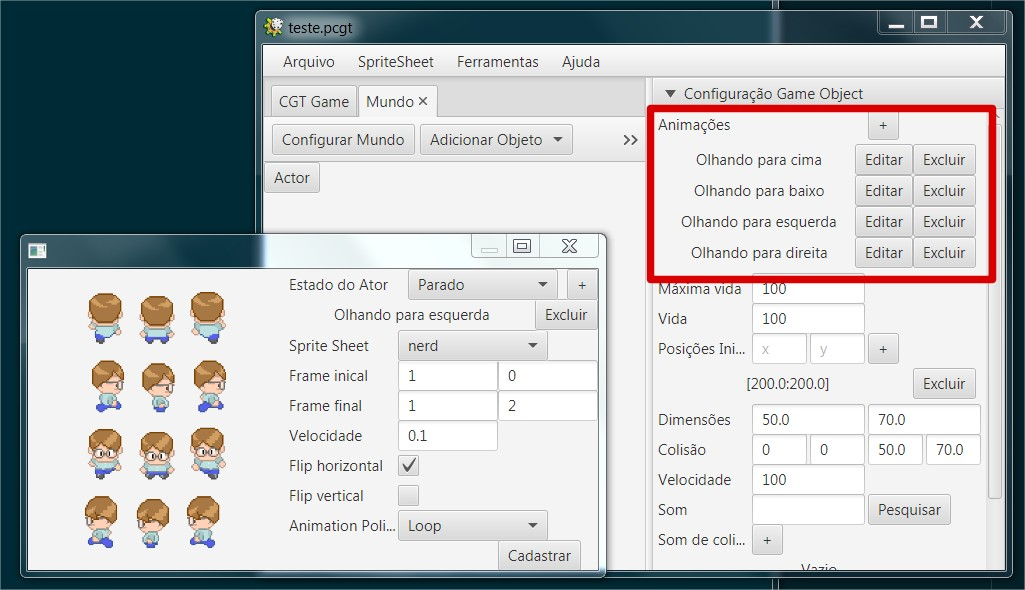
\includegraphics[width=\textwidth]{images/problema-2.jpg}
   \end{frame}

   \section{Descrição das melhorias}
   \subsection{Problema I - Organização dos objetos}
   \subsubsection{Descrição}
   \begin{frame}
      \frametitle{Organização dos objetos do jogo}
      \framesubtitle{Descrição do problema}
      \begin{itemize}
         \item Jogos possuem muitos objetos e são longos.
         \item Hierarquia entre objetos.
         \item As características importam na organização.
         \item Tipos de objetos:
            \begin{multicols}{2}
               \begin{itemize}
                  \item Mundo,
                  \item Ator,
                  \item Inimigo,
                  \item Opositor,
                  \item Bônus,
                  \item Projétil,
                  \item Tela,
                  \item Botão de tela,
                  \item Barra de vida e
                  \item Barra de munição.
               \end{itemize}
            \end{multicols}
      \end{itemize}
   \end{frame}

   \begin{frame}

      {\footnotesize
      \begin{tabular}{ l | p{7cm} }
         \textbf{Objeto} & \textbf{Descrição} \\
         \hline
         Mundo & Fase do jogo definindo o plano de fundo.  \\
         \hline
         Ator & Objeto controlado pelo jogador. \\
         \hline
         Inimigo & Objeto que causa dano ao ator e impede os objetivos dele. \\
         \hline
         Opositor & Objeto que impede ações do ator.  \\
         \hline
         Bônus & Objeto que promove bônus ao ator. \\
         \hline
         Projétil & Objeto que pode ser arremessado pelo ator. \\
         \hline
         Tela & Representa uma tela do jogo. \\
         \hline
         Botão de tela & Botão de uma tela do jogo. \\
         \hline
         Vida de um objeto & Mostra a quantidade de vida que um objeto possui. \\
         \hline
         Munição de um objeto & A quantidade de projéteis que o ator ainda pode arremessar. \\
      \end{tabular}}
   \end{frame}

   \begin{frame}
      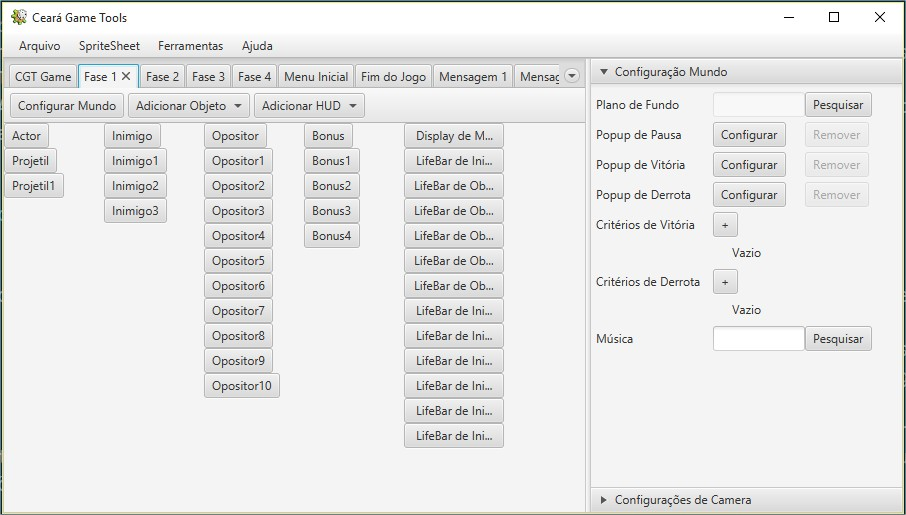
\includegraphics[width=\textwidth]{images/objetos_disposicao.jpg}
   \end{frame}

   \subsubsection{Resolução}
   \begin{frame}
      \frametitle{Organização de objetos no jogo}
      \framesubtitle{Resolução do problema}

      \begin{columns}[T]
         \begin{column}{0.48\textwidth}
            \begin{itemize}
               \item Árvore de objetos;
               \item Visão de tudo que existe no jogo;
               \item Objetos acessíveis a poucos cliques;
               \item Ocupa menor espaço na janela.
            \end{itemize}
         \end{column}
         \begin{column}{0.48\textwidth}
            \begin{center}
            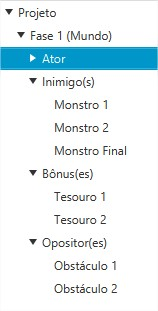
\includegraphics[width=0.48\textwidth]{images/arvore_objetos.jpg}
            \end{center}
         \end{column}
      \end{columns}
   \end{frame}

   \begin{frame}
      \begin{center}
         \begin{tabular}{| p{8cm} | l | }
            \hline
            \textbf{Item} & \textbf{Item superior} \\
            \hline
            Projeto & (Raiz) \\
            Mundo & Projeto \\
            Ator, Inimigos, Bônus(es), Opositor(es) & Mundo \\
            Projetil & Ator \\
            Barra de vida & Ator, Inimigo \\
            Munição & Projétil \\
            Tela & Projeto \\
            Botão de tela & Tela \\
            \hline
         \end{tabular}
      \end{center}
   \end{frame}

   \subsection{Problema II - Painéis de configuração}
   \subsubsection{Descrição}
   \begin{frame}
      \frametitle{Painéis de configuração}
      \framesubtitle{Problemas encontrados}
      \begin{itemize}
         \item Falta clareza;
         \item Valores possíveis (mínimo e máximo);
         \item Fluidez da aplicação;
         \item Mostrar o significado de cada propriedade ao usuário.
      \end{itemize}
   \end{frame}

   \begin{frame}
      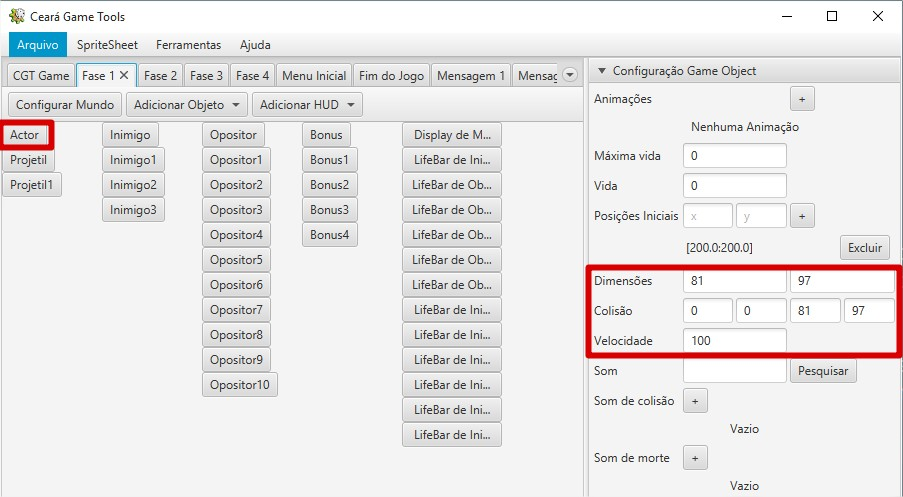
\includegraphics[width=\textwidth]{images/obj_dimensoes.jpg}
   \end{frame}

   \subsubsection{Resolução}
   \begin{frame}
      \frametitle{Painéis de configuração}
      \framesubtitle{Resolução do problema}

      \begin{itemize}
         \item Evitar diálogos (janelas que sobrepõem a janela principal);
         \item Interagir com demais áreas;
         \item Aprimorar os painéis da \texttt{ferramenta 1.0} para a \texttt{ferramenta 2.0} (exemplo configuração das animações de um objeto).
         \item Segregar as configurações dos objetos.
      \end{itemize}
   \end{frame}

   \begin{frame}
      \begin{center}
         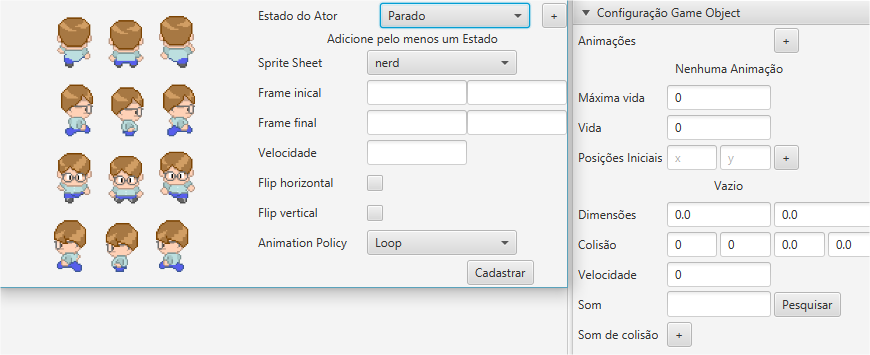
\includegraphics[width=0.9\textwidth]{images/add_animacao_1.png}
      \end{center}
   \end{frame}

   \begin{frame}
      \begin{center}
         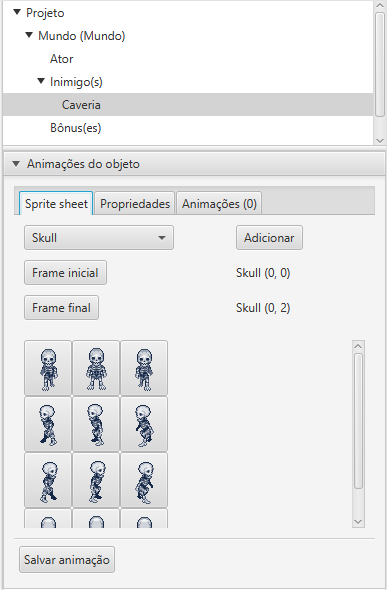
\includegraphics[width=0.38\textwidth]{images/add_animacao_2.png}
      \end{center}
   \end{frame}

   \subsection{Problema III - Ausência de pré visualização dos objetos}
   \subsubsection{Descrição}
   \begin{frame}
      \frametitle{Pré visualização}
      \framesubtitle{Problemas encontrados}
         \begin{itemize}
            \item Executar o jogo com muita frequência;
            \item Entender melhor as configurações feitas;
            \item A prévia contribui para problemas anteriores;
         \end{itemize}
   \end{frame}

   \begin{frame}
      \begin{center}
         \begin{tabular}{p{12em} | p{12em}}
            \textbf{Objeto(s)} & \textbf{Atributo(s)} \\
            \hline
            Mundo e tela do jogo & Plano de fundo \\
            \hline
            Ator, inimigo, bônus, opositor e projétil & Animações (\emph{spritesheet}), posição inicial, dimensões e área de colisão. \\
            \hline
            Botão de uma tela & Posição, dimensões, textura do botão normal e textura quando for pressionado.\\
            \hline
            Munição do projétil & Posição, dimensões e ícone. \\
            \hline
            Barra de vida de um objeto & Posição, dimensões, textura do preenchimento da barra e textura do plano de fundo. \\
         \end{tabular}
      \end{center}
   \end{frame}

   \subsubsection{Resolução}
   \begin{frame}
      \frametitle{Resolução do problema}
      \framesubtitle{Pré visualização}

      \begin{block}{Área de pré visualização}
         Espaço na ferramenta responsável por mostrar os objetos que foram criados, possibilitando que sejam visualizados pelo usuário.
      \end{block}

      \begin{itemize}
         \item Deve refletir com as configurações feitas;
         \item Deve estar sincronizado com a árvore de objetos;
         \item Deve ser fiel ao jogo;
      \end{itemize}

   \end{frame}

   \begin{frame}
      \begin{center}
         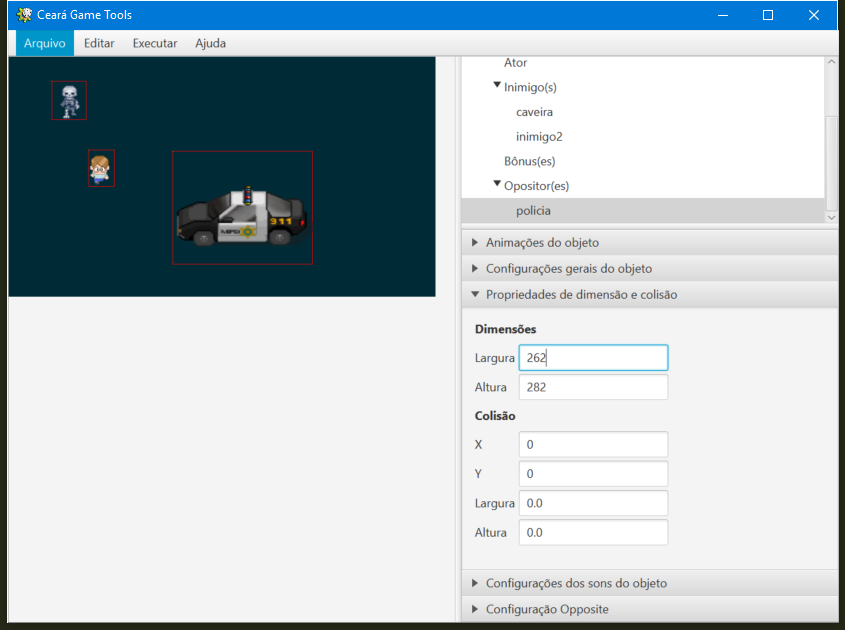
\includegraphics[width=0.9\textwidth]{images/preview2.png}
      \end{center}
   \end{frame}

   \section{Estudo de caso}
   \begin{frame}
   \end{frame}

   \section{Conclusão e trabalhos futuros}
   \begin{frame}
      \begin{center}
         Obrigado
      \end{center}
   \end{frame}

   \section{Referências}
   \begin{frame}[allowframebreaks]{Referências}
   \bibliography{references}
   \end{frame}

\end{document}
